\documentclass[12pt, a4paper]{report}
\usepackage[utf8]{inputenc}
\usepackage[T1]{fontenc}
\usepackage{hyperref}
\hypersetup{colorlinks=true, linkcolor=blue, filecolor=magenta, urlcolor=cyan,}
\urlstyle{same}
\usepackage{amsmath}
\usepackage{amsfonts}
\usepackage{amssymb}
\usepackage{graphicx}
\usepackage{enumitem}
\usepackage{geometry}
\usepackage[export]{adjustbox}
\usepackage{titlesec}
\geometry{lmargin=30mm}
\titleformat{\chapter}{\normalfont\huge}{\thechapter}{20pt}{\huge\bf}
\graphicspath{{images/}} %configuring the graphicx package
\title{Practica 1}
\author{Javier Izquierdo Hernández}
\date{\today}

\begin{document}
	\begin{titlepage}
		\centering
		{
\includegraphics[width=0.3\textwidth]{logo}\par}
		\vspace{1cm}
		{\bfseries\LARGE Universidad Rey Juan Carlos \par}
		\vspace{1cm}
		{\scshape\Large E.T.S. Ingeniería de Telecomunicación \par}
		\vspace{3cm}
		{\scshape\Huge Fundamentos de redes de ordenadores \par}
		\vspace{3cm}
		{\itshape\Large Práctica 6 \par}
		\vfill
		{\Large Autor: \par}
		{\Large Javier Izquierdo Hernández \par}
		\vfill
		{\Large \today \par}
	\end{titlepage}

\newpage
\renewcommand{\contentsname}{Contenidos}
\tableofcontents
\newpage

\begin{abstract}
Resumen En esta práctica se aprende el funcionamiento básico del DNS. Para su realización es necesario que descargues el escenario p6-lab.tgz a través del siguiente enlace: 
 https://mobiquo.gsyc.urjc.es/practicas/fro/p6.html 
 NOTA: Para realizar todas las capturas de esta práctica utiliza tcpdump tal y como venías usándolo en otras prácticas pero además añade la opción -n para que la propia aplicación tcpdump no solicite otras resoluciones adicionales al DNS para mostrar la información de forma más amigable.
\end{abstract}

\chapter{Introducción}
\begin{center}
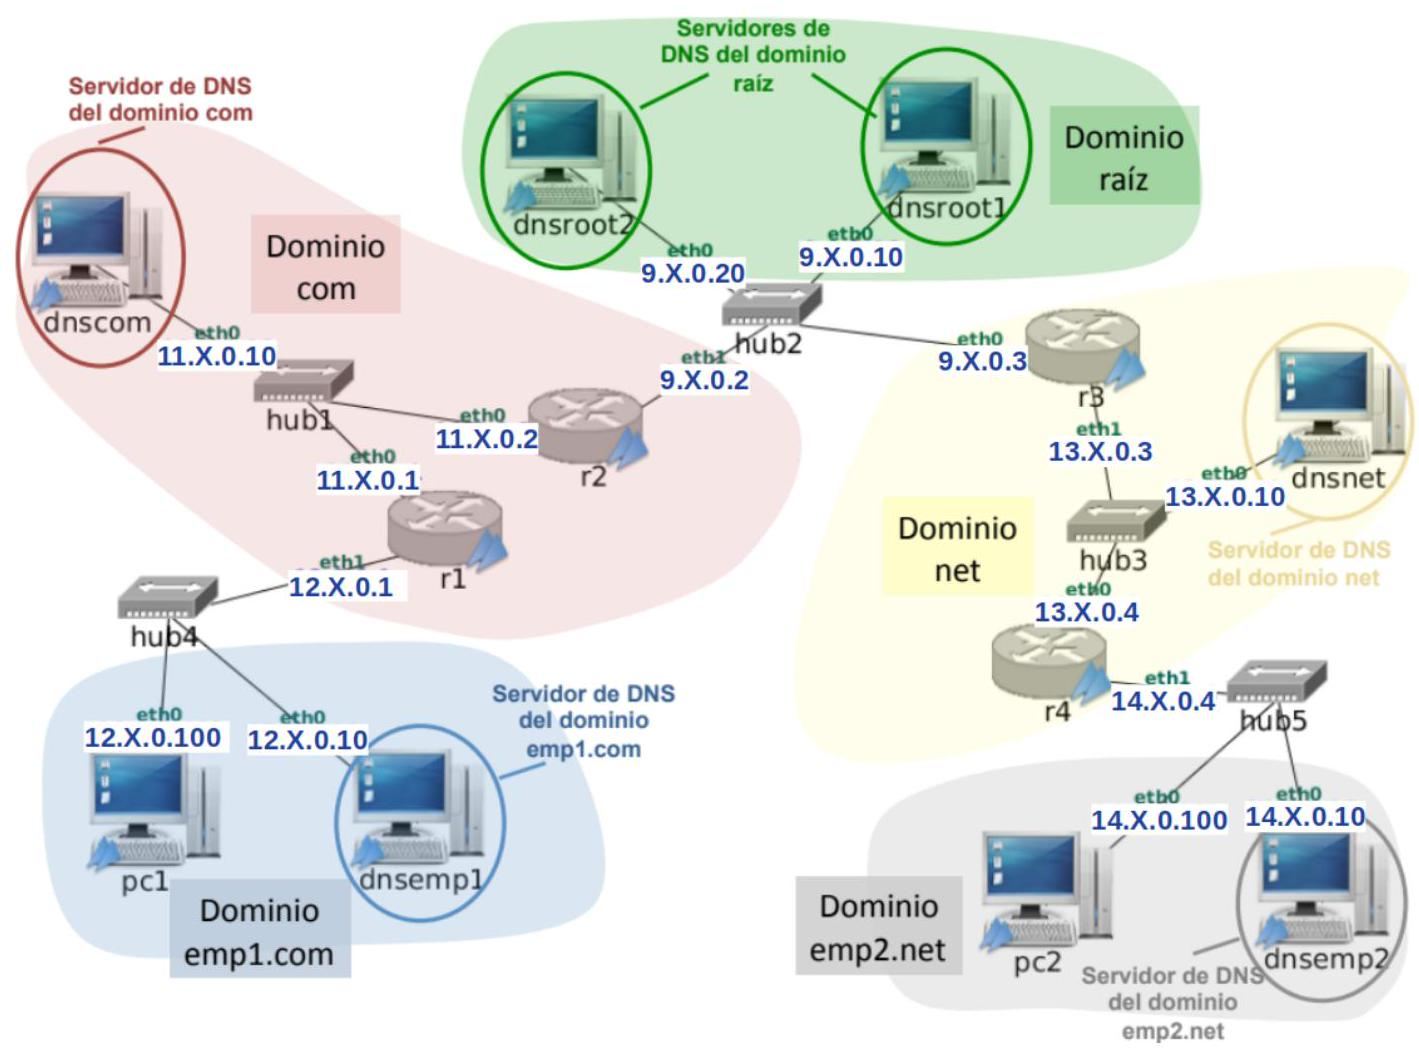
\includegraphics[max width=\textwidth]{2022_12_15_5d692d3f6b88770a0becg-1}
\end{center}

Figura 1: Escenario p6-lab

\chapter{Árbol de dominios}
El escenario de la práctica está formado por 4 routers y 8 máquinas. Dentro de este escenario existen los siguientes dominios (véase la figura 1 ):

\begin{itemize}
  \item Dominio raíz donde se encuentran las máquinas dnsroot1 y dnsroot2.

  \item Dominio com: donde se encuentran los routers r1 y r2 y la máquina dnscom. Por tanto, su nombre completo es $\mathrm{r} 1 . \mathrm{com}, \mathrm{r} 2 . \mathrm{com}$ y dnscom. com respectivamente.

  \item Dominio \href{http://emp1.com}{emp1.com}: donde se encuentran las máquinas pc1 y dnsemp1. Por tanto, su nombre completo es pc1. \href{http://emp1.com}{emp1.com} y dnsemp1. \href{http://emp1.com}{emp1.com} respectivamente.

  \item Dominio net: donde se encuentran los routers r3 y r4 y la máquina dnsnet. Por tanto, su nombre completo es $\mathrm{r} 3$. net, $\mathrm{r} 4$. net y \href{http://dnsnet.net}{dnsnet.net} respectivamente.

  \item Dominio emp2. net: donde se encuentran las máquinas pc2 y dnsemp2. Por tanto su nombre completo es: pc2. \href{http://emp2.net}{emp2.net} y dnsemp2. \href{http://emp2.net}{emp2.net} respectivamente.

\end{itemize}

\chapter{Servidores de DNS: Ficheros de configuración y mapas}
La siguiente tabla muestra las máquinas del escenario que son servidores de DNS:

\begin{center}
\begin{tabular}{|l|l|l|}
\hline
Máquina & Descripción & Ficheros de configuración \\
\hline\hline
dnsroot1 & Servidor de nombres raíz & letc/bind/named.conf /etc/bind/db.root \\
\hline
dnsroot2 & Servidor de nombres raíz & letc/bind/named.conf letc/bind/db.root \\
\hline
dnscom & Servidor de nombres del dominio com & letc/bind/named.conf letc/bind/db.root letc/bind/db.com \\
\hline
dnsemp1 & Servidor de nombres del dominio emp1.com & letc/bind/named.conf /etc/bind/db.root letc/bind/db.emp1.com \\
\hline
dnsnet & Servidor de nombres del dominio net & letc/bind/named.conf letc/bind/db.root letc/bind/db.net \\
\hline
dnsemp2 & Servidor de nombres del dominio emp2.net & letc/bind/named.conf /etc/bind/db.root letc/bind/db.emp2.net \\
\hline
\end{tabular}
\end{center}

En esas máquinas se ha utilzado el paquete bind9 para instalar el servidor de DNS. En la tabla anterior aparecen especificados los ficheros de configuración más importantes en cada servidor. Todos ellos se encuentran en la carpeta /etc/bind de cada máquina virtual).

Para ver el contenido de un ficheros en una máquina virtual puedes utilizar la la orden less en la máquina que contiene dicho fichero:

less 

Así, por ejemplo, para el ver el mapa del dominio emp2. net, tienes que escribir en la ventana de terminal de la máquina dnsemp2. emp2 .net la orden:

dnsemp2 :\# less /etc/bind/db.emp2.net

Mientras usas less puedes moverte adelante y atrás por el contenido del fichero utilizando las flechas del cursor. Para salir de less pulsa la tecla q (quit). A continuación se explica el propósito y contenido de estos ficheros de configuración de los servidores de DNS:

\begin{itemize}
  \item named.conf:
\end{itemize}

Fichero con la configuración general del servidor de DNS: lista de dominios (zonas) que se sirven y nombres de los ficheros que contienen los mapas de esos dominios. Como ejemplo se muestra a continuación parte del contenido de este fichero en el servidor dnscom:

\begin{center}
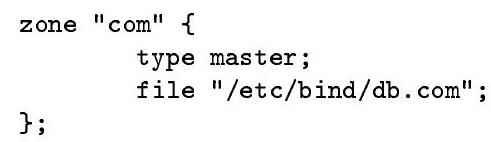
\includegraphics[width=100mm]{2022_12_15_5d692d3f6b88770a0becg-3}
\end{center}

El contenido de este fichero indica que la máquina donde se encuentra dicho fichero, dnscom, es servidor maestro $^{1}$ del dominio .com y que el fichero que almacena el mapa de ese dominio es /etc/bind/db.com

\begin{itemize}
  \item db.root:
\end{itemize}

Mapa del dominio raíz de DNS (dominio "."), almacenado en los servidores de dicho dominio (dnsroot1 y dnsroot2). Su contenido en dnsroot1 es:

\begin{center}
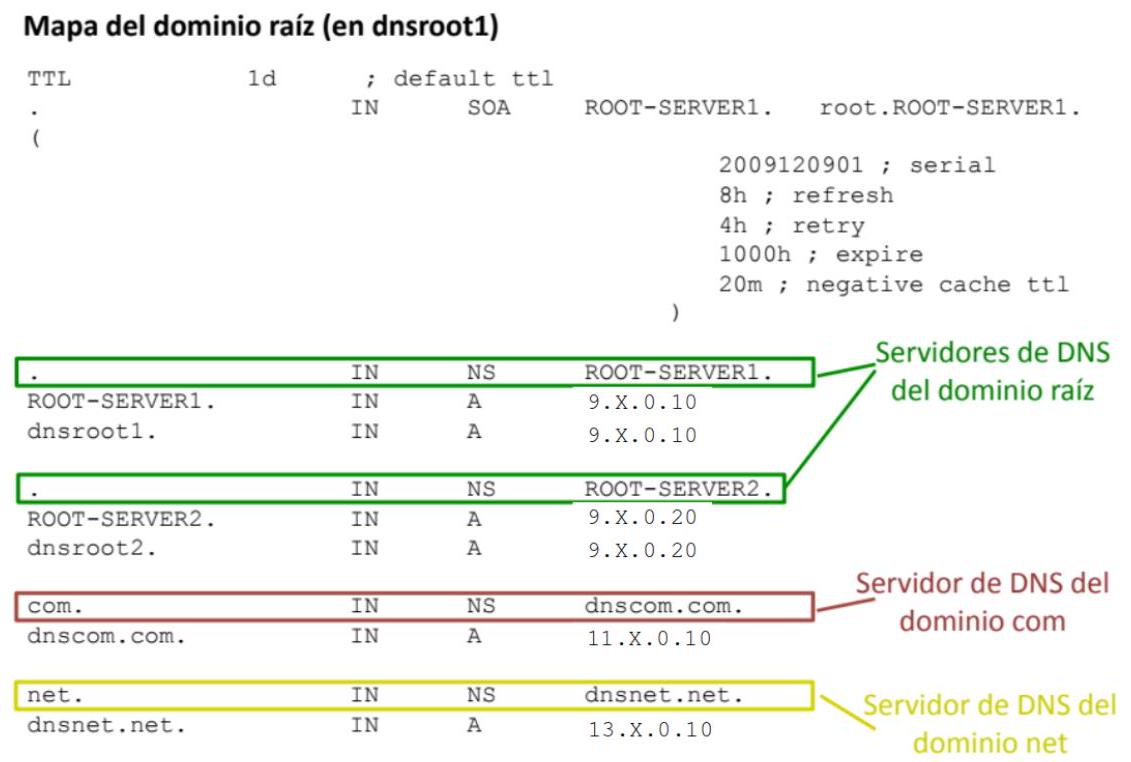
\includegraphics[width=\textwidth]{2022_12_15_5d692d3f6b88770a0becg-3(1)}
\end{center}

En dicho mapa se encuentra la relación de subdominios directos del raíz, que en este escenario son .com y .net, junto con el nombre e IP de los servidores de ese subdominio.

En dnsroot2 el fichero db .root tendrá un contenido similar, con leves cambios en el registro SOA.

En el resto de servidores (dnscom, dnsnet, dnsemp1 dnsemp2), pese a que no son servidores del dominio raíz, también existe este fichero db.root. En estos casos el fichero contiene simplemente la lista de las IPs de servidores del dominio raíz. Esta información la necesitan los servidores para iniciar la cadena de búsqueda de nombres que no conozcan.

NOTA: El contenido de este fichero es considerado "provisional" por los servidores, y la primera vez que un servidor tenga que enviar un mensaje a un servidor raíz sacado de este dichero, le enviará también una consulta adicional preguntando la lista de servidores del dominio raíz, por si hubiera habido cambios.

${ }^{1}$ No estudiamos en este tema la diferencia entre servidores maestros y esclavos de un dominio, todos los servidores de un dominio que estudiaremos serán servidores maestros En esos servidores (dnscom, dnsnet, dnsemp1 dnsemp2) el contenido de db.root es:

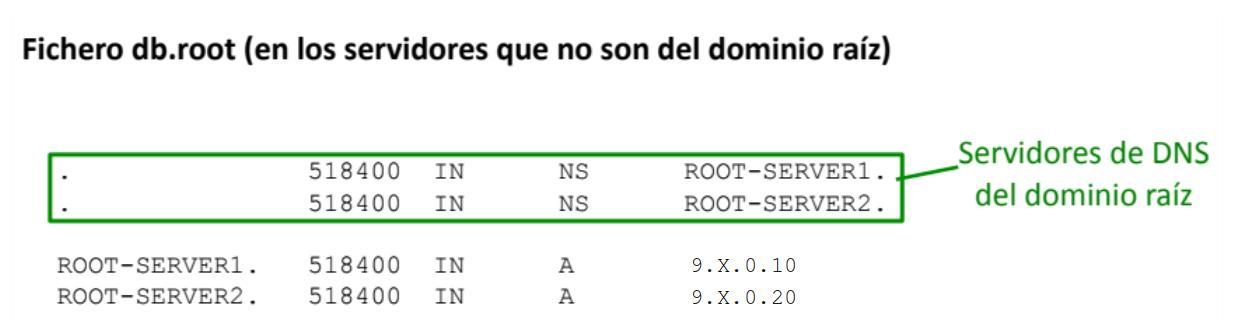
\includegraphics[width=\textwidth]{enunciado2}

\begin{itemize}
  \item $\mathrm{db} . *$ :
\end{itemize}

Los ficheros que empiezan por $\mathrm{db}$. contienen el mapa del dominio que sirve un determinado servidor.

Así, por ejemplo, el servidor de DNS del servidor dnsemp1 sirve el mapa del dominio emp1 . com y por tanto, tiene el fichero /etc/bind/db .emp1.com que almacena el mapa del dominio \href{http://emp1.com}{emp1.com}, cuyo contenido es

\begin{center}
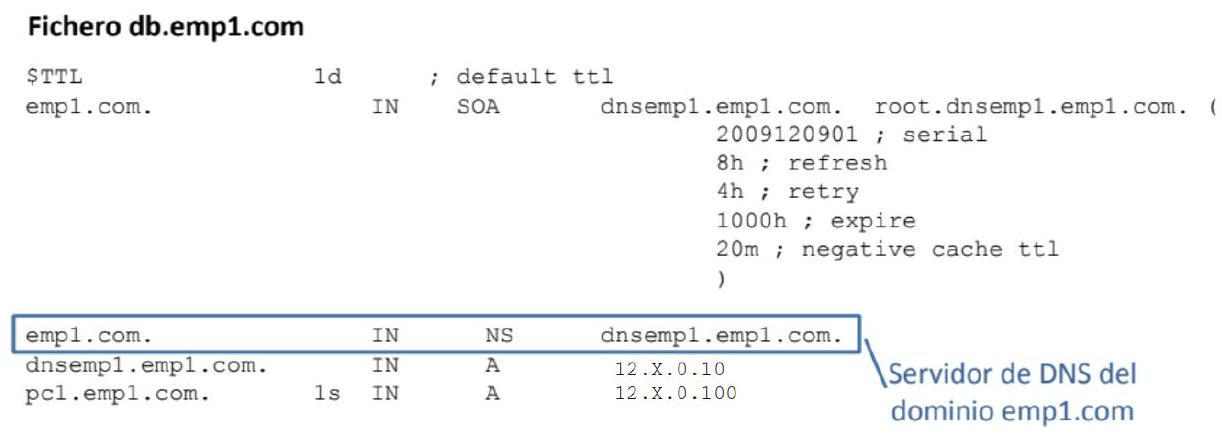
\includegraphics[max width=\textwidth]{2022_12_15_5d692d3f6b88770a0becg-4}
\end{center}

\chapter{Caché de un servidor DNS}
Para ver el contenido de la caché de DNS de un servidor de DNS, ejecuta en su máquina la siguientes dos órdenes, una detrás de otra:

rndc dumpdb - cache

less /var/cache/bind/named\_dump.db

La primera órden vuelca el contenido de la caché de DNS del servidor en el fichero /var/cache/bind/named\_dump.db, y la segunda te permite consultar su contenido. Un ejemplo de contenido de una caché en un momento dado puede ser:

\begin{center}
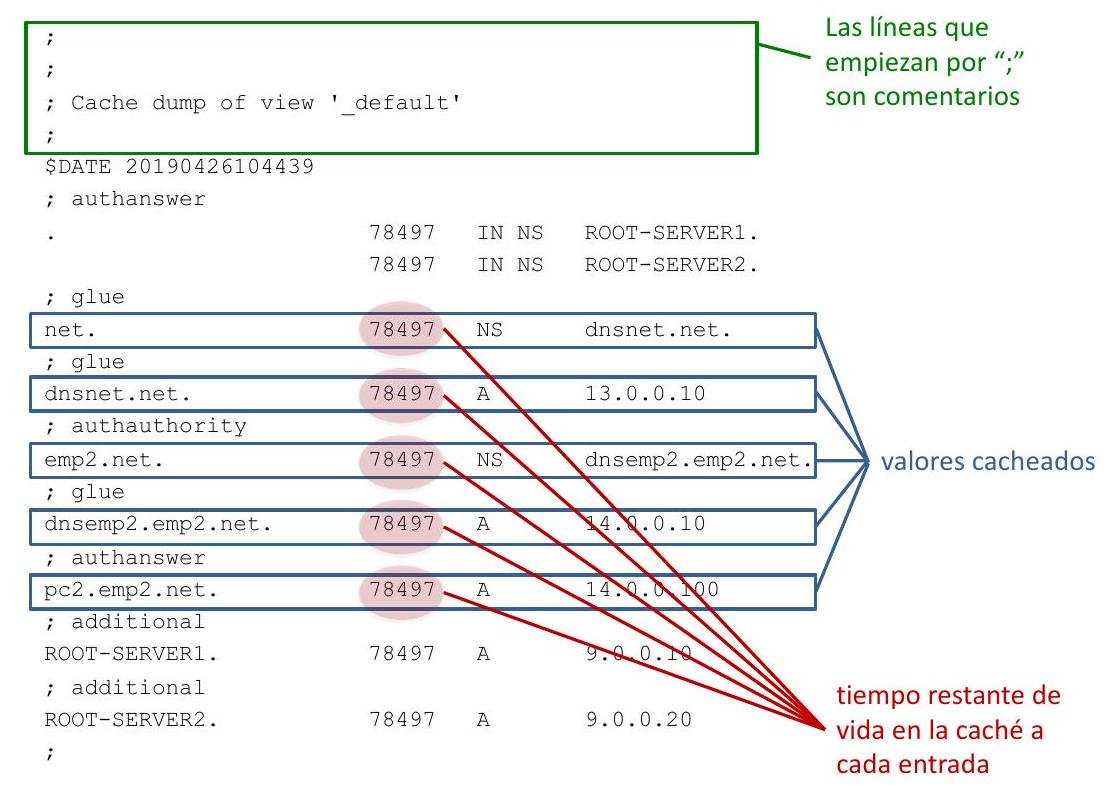
\includegraphics[max width=\textwidth]{2022_12_15_5d692d3f6b88770a0becg-4(1)}
\end{center}

Ten en cuenta que cada vez que quieras ver de nuevo el contenido de la caché debes ejecutar primero la orden rndc para actualizar el contenido del fichero, y después ejecutar la orden less para mostar el nuevo contenido del fichero.

Para borrar todos los contenidos de la caché de DNS de un servidor, ejecuta en su máquina la orden:

rndc flush

\chapter{Configuración del servidor de nombres de cada máquina cliente}
Todas las máquinas del escenario están configuradas de forma que cuando quieran saber la IP que se corresponde con un nombre, primero consultarán su fichero local /etc/hosts, y si no encuentran la respuesta, consultarán su servidor de DNS.

Cada máquina tiene configurado su servidor de DNS en su fichero /etc/resolv . conf, de la siguiente forma:

\begin{itemize}
  \item Las máquinas dnsroot1 y dnsroot2 tienen cada una configurado como servidor de DNS a ella misma.

  \item Las máquinas pc1 y dnsemp1 tienen configurado como servidor de DNS a dnsemp1.

  \item Las máquinas pc2 y dnsemp2 tienen configurado como servidor de DNS a dnsemp2.

  \item La máquina dnscom y los routers r1 y r2 tienen configurado como servidor de DNS a dnscom.

  \item La máquina dnsnet y los routers r3 y r4 tienen configurado como servidor de DNS a dnsnet.

\end{itemize}

\chapter{Programa host}
Para consultar al DNS puede utilizarse la orden host, herramienta que permite realizar consultas a un servidor de DNS. Utilizaremos este programa de la siguiente forma:

host <nombreDeMáquina>

El programa host mostrá la dirección IP asociada a <nombreDeMáquina>, como resultado de haber consultado al servidor de DNS que tenga configurado la máquina donde se ejecuta el programa.

NOTA IMPORTANTE: El programa host consulta directamente al DNS, sin mirar nunca el fichero /etc/hosts, independientemente de la configuración de la máquina. El resto de órdenes como ping, traceroute, etc, utilizan dicho fichero, y con la configuración del escenario, primero mirarán en el /etc/hosts y luego interrogarán al DNS.

\chapter{Formato de los mensajes de DNS}
El formato de mensaje de DNS tiene muchos campos. Para la realización de esta práctica ten a mano para consultar las transparencias 36-38 del tema de teoría que contienen, en el formato utilizado por wireshark, los campos más importantes de los mensajes, que son los que debes intentar localizar en las capturas.

\chapter{Resolución de nombres}
Arranca las máquinas del escenario definido en DNS-lab de una en una y responde a las siguientes preguntas:

\begin{enumerate}
  \item Imagina qué ocurriría si la máquina pc1 ejecuta host pc2.emp2.net. ¿Cuántos mensajes de DNS se generarían y entre qué máquinas? Es importante que consideres que es la primera consulta que se realiza en ese escenario (las cachés de los servidores de DNS están vacías).
  
  Mandará 10 datagramas DNS:
  \begin{itemize}
  	\item 2 entre pc1 y dnsemp1, en el primero le pregunta por la dirección, y el segundo es la respuesta
  	\item 4 entre dnsemp1 y dnsroot1
  	\item 2 entre dnsemp1 y dnsnet
  	\item 2 entre dnsemp1 y dnsemp2
  \end{itemize}

  \item Ejecuta la instrucción anterior en pc1, realizando previamente una captura de tráfico en r1(eth1) para ver todos los mensajes de DNS generados. Almacena los paquetes de la captura en el fichero p6-dns-01.cap ejecutando el comando con la opción -n :

	tcpdump -n -s $0-i$ <interfaz $\rangle-\mathrm{w}\langle\text { fichero }\rangle$.

  \item Observa en la captura cómo el mensaje de consulta que envía pc1 tiene activado el flag Recursion desired para que la consulta sea recursiva y los mensajes de consulta que envía dnsemp1 no tienen activado el flag Recursion desired para que la consulta se realice de forma iterativa.
  
  	\includegraphics*[width=128mm, scale=0.5, center]{ejercicio1}
	\includegraphics*[width=128mm, scale=0.5, center]{ejercicio2}

  \item Observa en la/s captura/s el valor TTL (Time To Live) de la respuesta obtenida en pc1. NOTA: No confundir el TTL de los mensajes de DNS de respuesta con el TTL de cabecera IP. En esta práctica siempre hablamos del TTL de los mensajes de DNS.
  
  Tiene el valor de 1 día.

  \item Para cada uno de los mensajes de respuesta que observes, explica qué línea/s de cada uno de los mapas de dominio (db.*) proporcionan la información que viaja en dichos mensajes (registros A o registros NS). Para ello mira el contenido de los ficheros de dichos mapas.
  
  \begin{itemize}
  	\item En el mensaje de respuesta a pc1 desde dnsemp1, la respuesta viene proporcionada por la pregunta a los servidores root encontrados en el fichero db.root en la línea 4, ya que este es el primero.
	\item En el mensaje de respuesta a dnsemp1 desde dnsroot1, se usa la línea 21-22 del fichero db.root
	\item En el mensaje de respuesta a dnsemp1 desde dnsnet, se usa la línea 18-19 del fichero db.net
	\item En el mensaje de respuesta a dnsemp1 desde dnsemp2, se usa la línea 13-14 del fichero db.emp2.net
  \end{itemize}

  \item Supón que ocurriría si después de haber realizado la consulta anterior, en pc1 se solicita de nuevo la resolución de pc2.emp2.net. ¿Cuántos mensajes de DNS se generarían y entre qué máquinas? ¿Por qué?
  
  Solo se realizan 2 mensajes, porque pc1 ya tiene la dirección de pc2.emp2.net. en caché.

  \item Ejecuta la resolución anterior en pc1, realizando de nuevo una captura en $r 1$ (eth1) y guardando su contenido en el fichero p6-dns-02.cap para ver todos los mensajes de DNS generados.

  \item Explica el valor TTL (Time To Live) de la respuesta obtenida en pc1. Compáralo con el valor obtenido en el apartado 2.
  
  Es de 86242 en vez de 86400 segundos del apartado 2, esto puede ser el tiempo que ha pasado desde que se han realizado las capturas, es decir desde que pc1 ha recibido la información de consultar la Ip de pc2.

  \item Imagina qué mensajes de DNS se generarían y entre qué máquinas si en pc2 se pide la resolución de pc1.emp1.com.
  
  Mandará 10 datagramas DNS:
	\begin{itemize}
		\item 2 entre pc2 y dnsemp2, en el primero le pregunta por la dirección, y el segundo es la respuesta
		\item 4 entre dnsemp2 y dnsroot2
		\item 2 entre dnsemp2 y dnscom
		\item 2 entre dnsemp2 y dnsemp1
	\end{itemize}
  \item Ejecuta la resolución anterior en pc2, realizando una captura de tráfico en la interfaz $r 4$ (eth1) para ver todos los mensajes de DNS generados y guarda su contenido en el fichero p6-dns-03. cap.

  \item Consulta la caché de DNS en el servidor de DNS de pc2, dnsemp2. Explica su contenido.
  
	\includegraphics*[width=128mm, scale=0.5, center]{ejercicio3}
	
  En estos momentos tiene guardada la Ip de los servidores root, de .com y de .emp1.com

  \item Supón que ocurriría si después de haber realizado la consulta anterior, en pc2 se solicita de nuevo la resolución de pc1. emp1. com. ¿Cuántos mensajes de DNS se generarían y entre qué máquinas? ¿Por qué?
  
  Se deberían generar 2 datagramas DNS entre pc1 y pc2

  \item Ejecuta la resolución anterior en pc2, realizando una captura tráfico en la interfaz r4(eth1) para ver todos los mensajes de DNS generados y guarda su contenido en el fichero p6-dns-04.cap. Explica lo sucedido comparado con lo ocurrido en el apartado 7.
  
  Nuestra suposición del apartado anterior ha sido errónea porque la caché dns de pc2 no tenía la dirección Ip de pc1, por lo que le ha preguntado a emp2, que sí la tenía en caché.

  \item Consulta la caché de DNS en el servidor de DNS de pc1, dnsemp1. Explica su contenido.

  En estos momentos tiene guardada la Ip de los servidores root, de .net, de .emp2.net y de pc2.emp2.net

	\includegraphics*[width=128mm, scale=0.5, center]{ejercicio4}

  \item Imagina qué ocurriría si después de haber realizado las consultas anteriores, en pc1 se solicita la resolución de $r 4$.net. ¿Cuántos mensajes de DNS se generarían y entre qué máquinas?
  
  Mandará 4 datagramas DNS:
	\begin{itemize}
		\item 2 entre pc1 y dnsemp1, en el primero le pregunta por la dirección, y el segundo es la respuesta
		\item 2 entre dnsemp1 y dnsnet
	\end{itemize}

  \item Ejecuta la resolución anterior en pc1, realizando una captura tráfico en la interfaz r1(eth1) para ver todos los mensajes de DNS generados y guarda su contenidos en p6-dns-05.cap.
  \item El nombre r4. net tiene asociadas las dos direcciones IP del router r4. Comprueba que al solicitar la resolución de $r 4$. net sucesivas veces en pc1, el orden en el que se obtienen las direcciones IP de r4 es aleatorio.
  
  Si lo es, a veces aparecen en un orden y otras veces en el contrario.

  \item Imagina qué ocurriría en cada uno de los siguientes casos:


	\begin{enumerate}[label=\alph*]
		\item En pc1 se ejecuta la orden ping -n pc200.emp1.com.
		\item En pc1 se ejecuta la orden ping -n pc200.emp2.net.
		\item En pc1 se ejecuta la orden ping -n pc20.emp2.net.
	\end{enumerate}
	
	Ten en cuenta que ahora no vas a usar la orden host, que interroga directamente al DNS, sino una aplicación normal, ping, que usará la configuración de la máquina. Lo que significa que primero se buscará el nombre en el fichero /etc/hosts y si ahí no aparece, se preguntará al servidor de DNS.
	
	NOTA: la opción -n en el ping, igual que en el tcpdump o en traceroute, evita que el propio ping haga consultas adicionales al DNS para aportar más información a sus resultados. En esta práctica usa ping siempre con la opción $-\mathrm{n}$.
	
	Para cada uno de los casos responde a las siguientes cuestiones:
	\begin{enumerate}[label=\alph*]
		\item ¿Funcionaría el ping?
		\begin{itemize}
			\item ping -n pc200.emp1.com. : No
			\item ping -n pc200.emp2.net. : No
			\item ping -n pc20.emp2.net. : No
		\end{itemize}
		\item ¿Al ejecutar el ping puedes ver la dirección IP asociada al nombre? ¿En qué fichero o mapa está esa asociación de nombre e IP?
		\begin{itemize}
			\item ping -n pc200.emp1.com : Si, en pc1 host
			\item ping -n pc200.emp2.net : Si, en emp2 db.emp2.net
			\item ping -n pc20.emp2.net : No
		\end{itemize}
		\item ¿Cuántos mensajes de DNS se generarían y entre qué máquinas?
		\begin{itemize}
			\item ping -n pc200.emp1.com. : 0
			\item ping -n pc200.emp2.net. : 4 entre pc1, emp1 y emp2
			\item ping -n pc20.emp2.net. : 6 entre pc1, emp1 y emp2
		\end{itemize}
	\end{enumerate}


  \item Ejecuta las órdenes anteriores, realizando una captura de tráfico en cada caso:
  \begin{enumerate}[label=\alph*]
  	\item En pc1 se ejecuta la orden ping -n pc200. emp1. com y se captura tráfico en r1(eth1) guardando el tráfico en el fichero p6-dns-06 . cap.
  	\item En pc1 se ejecuta la orden ping -n pc200. emp2. net y se captura tráfico en r1 (eth1) guardando el tráfico en el fichero p6-dns-07. cap.
  	\item En pc1 se ejecuta la orden ping -n pc20.emp2. net y se captura tráfico en r1(eth1) guardando el tráfico en el fichero p6-dns-08. cap.
  \end{enumerate}

  \item Observando los ficheros de configuración de los servidores de DNS, indica qué ocurriría si en pc1 se solicita por segunda vez la resolución de pc20.emp2.net.
  
  Este preguntaría a emp1, por pc20.emp2.net, y este le contestaría que no existe ese nombre, porqué lo tiene guardado en la caché

  \item Ejecuta la resolución anterior en pc1, realizando una captura de tráfico en r1(eth1) y guardando su contenido en p6-dns-09. cap. Indica durante cuanto tiempo se obtendría esta/s misma/s captura/s.
  
  Esta captura será igual durante los próximos 20 minutos

\end{enumerate}

\end{document}